\documentclass{article}
\usepackage{tikz, comment}
\usepackage{pifont}
\usepackage{fontspec, pgfplots}
\usetikzlibrary{arrows, decorations.markings, decorations.pathreplacing}
\begin{comment}
:Title: Not defined yet
:Tags: pappus&#146;s theorem, theorem of pappus;moment;perimeter;arc length of a curve;difference quotient
:Prob: 0.4976;0.4784;0.4756;0.4706;0.4598
:Author: Prof.Hu Ji-shan, HKUST
:Slug: No name yet

Description Here.........
\end{comment}
\begin{document}\centering 

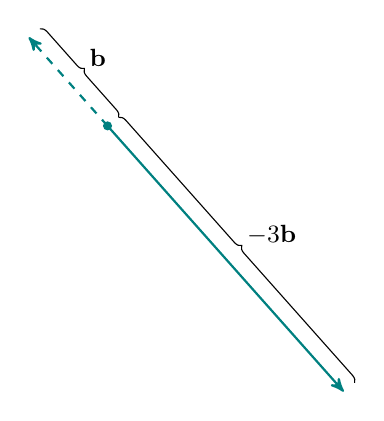
\begin{tikzpicture}[>=latex,xscale=.5*5, yscale=.5*5][font=\sf\small] 

\draw[dashed, teal, thick, ->, >=stealth'] (0, 0) -- (-0.4, 0.45);

\draw [decoration={brace,raise=2, mirror},decorate, xshift=1, yshift=0.7]
(0, 0) -- (-0.4, 0.45)node[black, right, midway, pos=0.5, xshift=2, yshift=7, scale=1]{$\bf b$}; %b

\draw[teal, thick, ->, >=stealth'] (0, 0) -- ({-0.4*(-3)}, {0.45*(-3)});
\draw [decoration={brace,raise=2},decorate, xshift=1, yshift=0.7]
(0, 0) -- ({-0.4*(-3)}, {0.45*(-3)})node[black, right, midway, pos=0.5, xshift=2, yshift=7, scale=1]{$-3\bf b$}; %-3b

\draw[teal, fill] (0,0) circle(0.02);

\end{tikzpicture}
\end{document}